\subsection{Stokes}
\subsubsection*{Plotten der Sinkgeschwindigkeiten}
Als ersten Schritt rechnet man die 5 erfassten Messreihen von Sinkzeiten \(t\) und Sinkstrecke \(s\) mit Fehler in die Geschwindigkeit um. Hierfür wird zuerst aus den pro Messreihe 5 erfassten Zeiten der Mittelwert \(\bar{t}\) (\cref{eq:arithmetisches_mittel}) berechnet. Da jedoch nur 5 Messwerte zur Verfügung stehen, wurde für \(\Delta \bar{t}\) nicht der Fehler des Mittelwerts genommen, sondern nur die klassische Standardabweichung \(\sigma\). Zusätzlich wurde quadratisch der Reaktionszeitfehler \(\Delta t=\qty{0.3}{\s}\) addiert (entsteht aus \(\sqrt{2}\cdot\qty{0.2}{s}\), den Reaktionszeiten beim Starten und Stoppen). 
\begin{equation}
    \Delta \bar{t}=\sqrt{\sigma(t_i)^2+(\qty{0.3}{\s})^2}
\end{equation}
Mithilfe des bekannten Fehlers \(\Delta s=\qty{0.005}{\cm}\) kannn nun die Geschwindigkeit mit Fehler berechnet werden:
\begin{equation}
    v=\frac{s}{t}\qquad \Delta v=\sqrt{\left(\frac{\Delta s}{t}\right)^2+\left(\frac{s\Delta t}{t^2}\right)^2}
    \label{eq:Geschwindigkeit}
\end{equation}
Zusätzlich werden mit der Ladenburgschen Korrektur \(\lambda v=(1+2.1\frac{r}{R})v\) versehene Geschwindgkeiten geplotted. Es war kein Fehler des Rohrradiuses \(R\) angegeben. Dieser wird deswegen als exakt angenommen. Fehler der korrigierten Geschwindigkeit ergibt sich zu:
\begin{equation}
\Delta (\lambda v)=\sqrt{\left(\Delta{v} \left(1 + \frac{2.1 r}{R}\right)\right)^{2} + \left(\Delta{r}\frac{2.1v}{R}\right)^{2}}
\end{equation}
Die Änderung von \(\Delta v\) ist nur minimal. An diese neuen Werte wurde eine Ursprungsgerade gefittet (siehe \cref{fig:Nr.1_Fit.png}). Mithilfe deren Steigung \(a\) kann nun die Viskosität \(\eta\) berechnet werden. Genutzt wurde hier die im Skript angegebene Dichte der Kügelchen: \(\rho_K=\qty{1.385(15)e3}{\kg\per\m\cubed}\) sowie die zur Raumtemperatur \(T=\qty{21.9(5)}{\degreeCelsius}\) passende PEG-Dichte (abgelesen in \cref{fig:DichtePEG.png}) \(\rho_F=\qty{1.1478(5)e3}{\kg\per\m\cubed}\).
\begin{gather}
    \eta=\frac{2g \left(\rho_{K}-\rho_{F}\right)}{9 a}\\
   \Delta \eta = \sqrt{\left(\frac{\Delta_{g} 2\left(-\rho_{F} +\rho_{K}\right)}{9 a}\right)^{2} + \left(- \frac{2 \Delta_{\rho_F} g}{9 a}\right)^{2} + \left(\frac{2 \Delta_{\rho_K} g}{9 a}\right)^{2} + \left(- \frac{\Delta_{a} g 2\left(-\rho_{F} +\rho_{K}\right)}{9 a^{2}}\right)^{2}}
\end{gather}
\begin{rb}
    \eta^\mathrm{Stokes}=\qty{0.268(0.004)}{\pascal\s}
\end{rb}

\xfigure{htbp}{width=\textwidth}{Nr.1_Fit.png}{}{unkorr. und korr. Sinkgeschwindigkeiten der Kügelchen mit Fitgerade}

\subsubsection*{Berechnen der \(v_{lam}\) Sinkgeschwindigkeiten}
Mithilfe \(\eta^\mathrm{Stokes}\) aus dem Fitergebnis (Steigung \(a\)) können nun die zu den Kugelradien gehörenden, theoretischen Sinkgeschwindigkeiten \(v_{lam}\) berechnet werden:
\begin{gather}
    v_{lam}=\frac{2 g r^{2} \left(- \rho_{F} + \rho_{K}\right)}{9 \eta}\\
    \frac{\Delta v_{lam}}{v_{lam}}=\sqrt{\frac{\Delta_{\eta}^{2}}{\eta^{2}} + \frac{\Delta_{g}^{2}}{g^{2}} + \frac{4 \Delta_{r}^{2}}{r^{2}} + \frac{\Delta_{\rho F}^{2}}{\left(\rho_{F} - \rho_{K}\right)^{2}} + \frac{\Delta_{\rho K}^{2}}{\left(\rho_{F} - \rho_{K}\right)^{2}}}
\end{gather}

\begin{table}[htb]
  \centering
  \caption{korrigierte Geschwindigkeiten}
  \begin{tabularx}{\textwidth}{ZZZ}
    \toprule
        r[\unit{\milli\m}]&v[\unit{\m\per\s}]&v_{lam}[\unit{\m\per\s}]\\\midrule
        \num{4.5}&\num{0.0377(0.0009)}&\num{0.0390(0.0007)}\\
        \num{4.0}&\num{0.031(0.0009)}&\num{0.0309(0.0006)}\\
        \num{3.5}&\num{0.024(0.0006)}&\num{0.0236(0.0005)}\\
        \num{3.0}&\num{0.0173(0.0007)}&\num{0.0174(0.0004)}\\
        \num{2.5}&\num{0.0131(0.001)}&\num{0.01204(0.00024)}\\
        \num{2.0}&\num{0.0079(0.0009)}&\num{0.00771(0.00016)}\\
        \num{1.5}&\num{0.0048(0.0005)}&\num{0.00434(0.00011)}\\
        \num{1.0}&\num{0.00203(0.00021)}&\num{0.00193(0.00006)}\\
        \num{0.5}&\num{0.00062(0.00016)}&\num{0.00049(0.00003)}\\
    \bottomrule
  \end{tabularx}
\label{table:lamGeschw}  
\end{table}
\newpage

In der folgenden Grafik sieht man dann nochmal schön, dass die Werte \(v_{lam}\) perfekt auf der Ausgleichsgeraden liegen, da sie mithilfe deren Steigung berechnet wurden.
\xfigure{htbp}{width=\textwidth}{Nr.1_Fitmitlam.png}{}{Eintragen der unzähligen Werte}

\subsubsection*{Reynoldszahl}
\begin{gather}
    Re=\frac{2 r \rho_{F} v}{\eta}\\
    \frac{\Delta Re}{Re}=\sqrt{\frac{\Delta_{\eta}^{2}}{\eta^{2}} + \frac{\Delta_{r}^{2}}{r^{2}} + \frac{\Delta_{\rho F}^{2}}{\rho_{F}^{2}} + \frac{\Delta_{v}^{2}}{v^{2}}}
    \label{eq:Reynolds}
\end{gather}
Das Verhältnis \(\frac{v}{v_{lam}}\) wird nun gegen \(log(Re)\) aufgetragen, die Reynoldszahlen \(Re\) wurden durch die obigen Formeln (nach \cref{eq:reynolds}) berechnet. Der Fehler des Geschwindigkeitsverhältnisses ergibt sich mit:
\begin{equation}
    \Delta\left(\frac{v}{v_{lam}}\right)=\sqrt{\left(\frac{\Delta v}{v_{lam}}\right)^2+\left(\frac{v\Delta v_{lam}}{v_{lam}^2}\right)^2}
\end{equation}

\xfigure{htbp}{width=\textwidth}{Nr.1_Reynoldszahl.png}{}{verzweifeltes Extrahieren der Grenze von laminarer zu turbulenter Strömung}
Als kritische Reynoldszahl wird aus \cref{fig:Nr.1_Reynoldszahl.png} abgeschätzt:
\begin{rb}
    Re^\mathrm{krit}=\num{0.246(50)}
\end{rb}

\FloatBarrier\subsection{Hagen-Poiseuille}
Mithilfe des Kapillarrohrs und einem dieses durchfließenden Volumenstroms kann die Viskosität auf die Weise von Hagen-Poiseuille berechnet werden, siehe \cref{eq:final_eta_hup}. Hier wird zuerst die Druckdifferenz mit dem hydrostatischen Druck \(p\) ausgedrückt (PFFFFTTT):
\begin{equation}
   p=\rho_{F}gh \qquad \Delta p=p\cdot\sqrt{\left(\frac{\Delta_h}{h}\right)^2+\left(\frac{\Delta\rho_F}{\rho_F}\right)^2+\left(\frac{\Delta g}{g}\right)^2}
\end{equation}
Dieser berechnet sich mit \(g=\qty{9.80984(2)}{\m\per\s\squared}\), \(h=\qty{0.540}{\m}\) zu \(\underline{p=\qty{6079.0(90)}{\pascal}}\). Da sowohl das große Rohr und die Kapillare offen sind, liegt an beiden der Atmosphärendruck an, welcher sich in der Druckdifferenz rauskürzt. 
Die Messdaten \(V(t)\) aus dem \hyperref[sec:Messprotokoll]{Messprotokoll} lassen sich nun durch Berechnen des Mittelwerts von \(\frac{\diff V}{\diff t}=\dot{V}\) (jedoch Auslassen des Werts \(V=\qty{5}{\milli\l}\)) in \cref{eq:final_eta_hup} einsetzen. Die Werte \(R=\qty{1.50(1)}{\milli\m}\) und \(L=\qty{100.0(5)}{\milli\m}\) sind im Skript angegeben. Nach Berechnen des Fehlers ergibt sich:
\begin{equation}
    \Delta \eta = \eta\sqrt{\frac{\Delta_{L}^{2}}{L^{2}} + \frac{\Delta \dot{V}^{2}}{\dot{V}^{2}} + \frac{\Delta_{p}^{2}}{p^{2}} + \frac{16 \Delta_{r}^{2}}{r^{2}}}
\end{equation}
\begin{rb}
    \eta^\mathrm{Hagen-Poiseuille}=\qty{0.261(17)}{\pascal\s}
\end{rb}
\paragraph{Reynolszahl:}
Wie schon bei Stokes geschehen, wird nun auch die Reynoldszahl mit \cref{eq:Reynolds} berechnet. Für \(v\) wird die mittlere Geschwindigkeit \(\bar{v}=\frac{\dot{V}}{\pi R^2}\) eingesetzt, \(r\) ist der Durchmesser \(R\) der Kapillare. Somit erhält man:
\begin{equation}
    Re=\frac{2\rho_F\dot{V}}{\pi\eta R} \qquad \Delta Re=Re\cdot\sqrt{\frac{\Delta_{L kap}^{2}}{L_{kap}^{2}} + \frac{\Delta_{dVdt}^{2}}{dVdt^{2}} + \frac{\Delta_{p}^{2}}{p^{2}} + \frac{16 \Delta_{r kap}^{2}}{r_{kap}^{2}}}
\end{equation}
\begin{rb}
    Re^\mathrm{Hagen-Poiseuille}=\num{0.109(0.011)}
\end{rb}
Damit liegt die Reynoldszahl für die vorliegenden Charakteristika (PEG-Dichte \(\rho_F\), Rohrdurchmesser \(2r\) und Strömungsgeschwindigkeit \(v\)) deutlich unter der kritischen Reynoldszahl (\(Re_{kr}=\num{2300}\) einer Rohrströmung) und wir können folglich tatsächlich von laminarer Strömung ausgehen, die Verwendung des Hagen-Poiseuille-Gesetzes ist also gerechtfertigt.

\subsection{Vergleich der Viskositäten}
Die Ergebnisse der zwei Versuchsmethoden werden hier verglichen: 
\begin{table}[htb]
  \centering
  \caption{Vergleich der berechneten Viskositäten}
  \begin{tabularx}{\textwidth}{ZZZ}
    \toprule
       \eta^\mathrm{Stokes}[\unit{\pascal\s}]&\eta^\mathrm{Hag.-Pois.}[\unit{\pascal\s}]&S[\sigma]\\
        \num{0.268(0.004)}&\num{0.261(17)}&\num{0.4}\\
    \bottomrule
  \end{tabularx}
\label{table:SIGGGGMAS}  
\end{table}

\newpage
\subsection{Differentialgleichung}
Aus dem Kräftegleichgewicht in \cref{eq:force_balance} lässt sich bestimmen, wie sich die Geschwindigkeit \(v(t)\) des Teilchens nach Eintauchen ändert. Dafür stellt man folgende Differentialgleichung auf:
\begin{equation}
\begin{aligned}    \underbrace{m\dot{v}}_{F_{res.}}&=\underbrace{\rho_KV_Kg}_{F_g} - \underbrace{\rho_F V_k g}_{F_a} - \underbrace{6\pi\eta r\,\lambda\,v_s}_{F_r}\\
    \dot{v}&=\underbrace{\frac{4\pi r^3(\rho_K-\rho_F)}{3m}}_{C}-\underbrace{\frac{6\pi\eta r}{m}}_{D}v=C-Dv
\end{aligned}
\end{equation}
Diese inhomogene DGL 1.Ordnung lässt sich mithilfe von Variation der Konstanten lösen: Die Lösung des homogenen Teils ist \(v_h=K(t)e^{-Dt}\), dieser Ansatz wird nun in die inhomogene DGL eingesetzt:
\begin{equation}
\begin{aligned}
    \frac{\diff}{\diff t}\left(K(t)e^{-Dt}\right)&=\dot{K}(t)e^{-Dt}-K(t)De^{-Dt}=C-DK(t)e^{-Dt}\\
    \dot{K}(t)e^{-Dt}&=C\\
    K(t)&=\int_{0}^{t}Ce^{Dt'}\diff t'=\frac{C}{D}e^{Dt}-\frac{C}{D}+v_0\\
\end{aligned}
\end{equation}
\(v_0\) entsteht aus den Integrationskonstanten. \\
Setzt man diese Lösung für \(K(t)\) nun wieder in die homogene Lösung ein, erhält man mit der Sinkgeschwindigkeit \(v_s=\frac{C}{D}\) das finale Ergebnis
\begin{rb}
    v(t)=\frac{C}{D}-\frac{C}{D}e^{-Dt}+v_0e^{-Dt}=v_s(1-e^{-Dt})+v_0e^{-Dt}
\end{rb}
Da es hier nur darum geht, ein Gefühl für die Größenordnungen zu bekommen, wird hier die Viskosität als \(\eta=\qty{0.2}{\pascal\s}\) angenommen. Man kann im Code verschiedene Startgeschwindigkeiten einstellen, und die Geschwindigkeit \(v(t)\) plotten lassen. Diese wird natürlich stark vom radiusabhängigen \(D\)-Wert beeinflusst, dieser skaliert mit \(r^{-2}\), somit sieht man in \cref{fig:Zusatz.png}, dass der Geschwindigkeitsabfalls für kleinere Radien zügiger von statten geht. Im Plot werden 3 berechnete Dinge angezeigt:
\begin{align*}
    v_\mathrm{beschleuniger}(t)&=v_0\cdot e^{-Dt}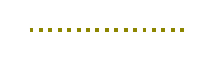
\begin{tikzpicture}
        \draw[olive,dotted,line width=1.4pt] (1cm,0) -- (3cm,0);
    \end{tikzpicture}\\
    v(t)&=v_s(1-e^{-Dt})+v_0\cdot e^{-Dt}\\
    t_\mathrm{schnitt}&=\frac{\ln{(\nicefrac{v_s}{v_0})}}{-a}
\end{align*}
Die Abbremszeit \(t_\mathrm{schnitt}\) wird berechnet, indem wie bei den Zusatzaufgaben\autocite{Dimitrij} vorgeschlagen wird, die relevante Größenordnung als \(v_s\) festgelegt wird, auf die \(v_\mathrm{beschl.}(t)\) absinken soll. 

\xfigure{t}{width=\textwidth}{Zusatz.png}{Abbremszeiten bei hoher Anfangsgeschw.}{Abbremszeiten für die Kugeln bei Startgeschwindigkeit}
\xfigure{!ht}{width=\textwidth}{Zusatzreal.png}{Abbremszeiten bei realistischer Anfangsgeschw.}{Abbremszeiten für die Kugeln bei Startgeschwindigkeit die zweite}
Man beobachtet, dass die Zeiten natürlich gemäß dem Logarithmus mit sinkender Startgeschwindigkeit immer kleiner werden, für unsere Messergebnisse spielt der Abbremsvorgang also keine signifikante Rolle. \\
\newpage
\xfigure{htbp}{width=0.6\textwidth}{geogebra-export.png}{\textit{Meme:} Erzählperspektive}{Langsam reicht es auch mit Memes. Je länger ich wach bin, desto ineffizienter wird alles}
